\documentclass[1p]{elsarticle_modified}
%\bibliographystyle{elsarticle-num}

%\usepackage[colorlinks]{hyperref}
%\usepackage{abbrmath_seonhwa} %\Abb, \Ascr, \Acal ,\Abf, \Afrak
\usepackage{amsfonts}
\usepackage{amssymb}
\usepackage{amsmath}
\usepackage{amsthm}
\usepackage{scalefnt}
\usepackage{amsbsy}
\usepackage{kotex}
\usepackage{caption}
\usepackage{subfig}
\usepackage{color}
\usepackage{graphicx}
\usepackage{xcolor} %% white, black, red, green, blue, cyan, magenta, yellow
\usepackage{float}
\usepackage{setspace}
\usepackage{hyperref}

\usepackage{tikz}
\usetikzlibrary{arrows}

\usepackage{multirow}
\usepackage{array} % fixed length table
\usepackage{hhline}

%%%%%%%%%%%%%%%%%%%%%
\makeatletter
\renewcommand*\env@matrix[1][\arraystretch]{%
	\edef\arraystretch{#1}%
	\hskip -\arraycolsep
	\let\@ifnextchar\new@ifnextchar
	\array{*\c@MaxMatrixCols c}}
\makeatother %https://tex.stackexchange.com/questions/14071/how-can-i-increase-the-line-spacing-in-a-matrix
%%%%%%%%%%%%%%%

\usepackage[normalem]{ulem}

\newcommand{\msout}[1]{\ifmmode\text{\sout{\ensuremath{#1}}}\else\sout{#1}\fi}
%SOURCE: \msout is \stkout macro in https://tex.stackexchange.com/questions/20609/strikeout-in-math-mode

\newcommand{\cancel}[1]{
	\ifmmode
	{\color{red}\msout{#1}}
	\else
	{\color{red}\sout{#1}}
	\fi
}

\newcommand{\add}[1]{
	{\color{blue}\uwave{#1}}
}

\newcommand{\replace}[2]{
	\ifmmode
	{\color{red}\msout{#1}}{\color{blue}\uwave{#2}}
	\else
	{\color{red}\sout{#1}}{\color{blue}\uwave{#2}}
	\fi
}

\newcommand{\Sol}{\mathcal{S}} %segment
\newcommand{\D}{D} %diagram
\newcommand{\A}{\mathcal{A}} %arc


%%%%%%%%%%%%%%%%%%%%%%%%%%%%%5 test

\def\sl{\operatorname{\textup{SL}}(2,\Cbb)}
\def\psl{\operatorname{\textup{PSL}}(2,\Cbb)}
\def\quan{\mkern 1mu \triangleright \mkern 1mu}

\theoremstyle{definition}
\newtheorem{thm}{Theorem}[section]
\newtheorem{prop}[thm]{Proposition}
\newtheorem{lem}[thm]{Lemma}
\newtheorem{ques}[thm]{Question}
\newtheorem{cor}[thm]{Corollary}
\newtheorem{defn}[thm]{Definition}
\newtheorem{exam}[thm]{Example}
\newtheorem{rmk}[thm]{Remark}
\newtheorem{alg}[thm]{Algorithm}

\newcommand{\I}{\sqrt{-1}}
\begin{document}

%\begin{frontmatter}
%
%\title{Boundary parabolic representations of knots up to 8 crossings}
%
%%% Group authors per affiliation:
%\author{Yunhi Cho} 
%\address{Department of Mathematics, University of Seoul, Seoul, Korea}
%\ead{yhcho@uos.ac.kr}
%
%
%\author{Seonhwa Kim} %\fnref{s_kim}}
%\address{Center for Geometry and Physics, Institute for Basic Science, Pohang, 37673, Korea}
%\ead{ryeona17@ibs.re.kr}
%
%\author{Hyuk Kim}
%\address{Department of Mathematical Sciences, Seoul National University, Seoul 08826, Korea}
%\ead{hyukkim@snu.ac.kr}
%
%\author{Seokbeom Yoon}
%\address{Department of Mathematical Sciences, Seoul National University, Seoul, 08826,  Korea}
%\ead{sbyoon15@snu.ac.kr}
%
%\begin{abstract}
%We find all boundary parabolic representation of knots up to 8 crossings.
%
%\end{abstract}
%\begin{keyword}
%    \MSC[2010] 57M25 
%\end{keyword}
%
%\end{frontmatter}

%\linenumbers
%\tableofcontents
%
\newcommand\colored[1]{\textcolor{white}{\rule[-0.35ex]{0.8em}{1.4ex}}\kern-0.8em\color{red} #1}%
%\newcommand\colored[1]{\textcolor{white}{ #1}\kern-2.17ex	\textcolor{white}{ #1}\kern-1.81ex	\textcolor{white}{ #1}\kern-2.15ex\color{red}#1	}

{\Large $\underline{12n_{0739}~(K12n_{0739})}$}

\setlength{\tabcolsep}{10pt}
\renewcommand{\arraystretch}{1.6}
\vspace{1cm}\begin{tabular}{m{100pt}>{\centering\arraybackslash}m{274pt}}
\multirow{5}{120pt}{
	\centering
	\includegraphics[width=112pt]{../../../GIT/diagram.site/Diagrams/png/2828_12n_0739.png}\\
\ \ \ A knot diagram\footnotemark}&
\allowdisplaybreaks
\textbf{Linearized knot diagam} \\
\cline{2-2}
 &
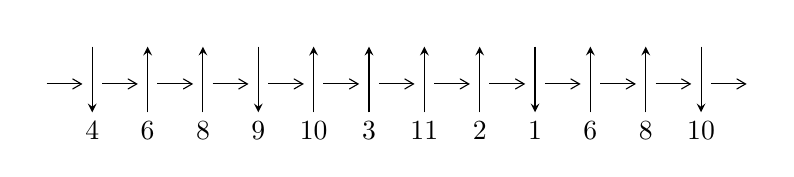
\begin{tikzpicture}[x=20pt, y=17pt]
	% nodes
	\node (C0) at (0, 0) {};
	\node (C1) at (1, 0) {};
	\node (C1U) at (1, +1) {};
	\node (C1D) at (1, -1) {4};

	\node (C2) at (2, 0) {};
	\node (C2U) at (2, +1) {};
	\node (C2D) at (2, -1) {6};

	\node (C3) at (3, 0) {};
	\node (C3U) at (3, +1) {};
	\node (C3D) at (3, -1) {8};

	\node (C4) at (4, 0) {};
	\node (C4U) at (4, +1) {};
	\node (C4D) at (4, -1) {9};

	\node (C5) at (5, 0) {};
	\node (C5U) at (5, +1) {};
	\node (C5D) at (5, -1) {10};

	\node (C6) at (6, 0) {};
	\node (C6U) at (6, +1) {};
	\node (C6D) at (6, -1) {3};

	\node (C7) at (7, 0) {};
	\node (C7U) at (7, +1) {};
	\node (C7D) at (7, -1) {11};

	\node (C8) at (8, 0) {};
	\node (C8U) at (8, +1) {};
	\node (C8D) at (8, -1) {2};

	\node (C9) at (9, 0) {};
	\node (C9U) at (9, +1) {};
	\node (C9D) at (9, -1) {1};

	\node (C10) at (10, 0) {};
	\node (C10U) at (10, +1) {};
	\node (C10D) at (10, -1) {6};

	\node (C11) at (11, 0) {};
	\node (C11U) at (11, +1) {};
	\node (C11D) at (11, -1) {8};

	\node (C12) at (12, 0) {};
	\node (C12U) at (12, +1) {};
	\node (C12D) at (12, -1) {10};
	\node (C13) at (13, 0) {};

	% arrows
	\draw[->,>={angle 60}]
	(C0) edge (C1) (C1) edge (C2) (C2) edge (C3) (C3) edge (C4) (C4) edge (C5) (C5) edge (C6) (C6) edge (C7) (C7) edge (C8) (C8) edge (C9) (C9) edge (C10) (C10) edge (C11) (C11) edge (C12) (C12) edge (C13) ;	\draw[->,>=stealth]
	(C1U) edge (C1D) (C2D) edge (C2U) (C3D) edge (C3U) (C4U) edge (C4D) (C5D) edge (C5U) (C6D) edge (C6U) (C7D) edge (C7U) (C8D) edge (C8U) (C9U) edge (C9D) (C10D) edge (C10U) (C11D) edge (C11U) (C12U) edge (C12D) ;
	\end{tikzpicture} \\
\hhline{~~} \\& 
\textbf{Solving Sequence} \\ \cline{2-2} 
 &
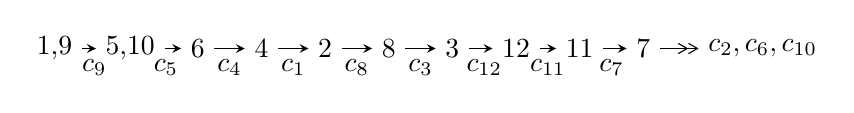
\begin{tikzpicture}[x=23pt, y=7pt]
	% node
	\node (A0) at (-1/8, 0) {1,9};
	\node (A1) at (17/16, 0) {5,10};
	\node (A2) at (17/8, 0) {6};
	\node (A3) at (25/8, 0) {4};
	\node (A4) at (33/8, 0) {2};
	\node (A5) at (41/8, 0) {8};
	\node (A6) at (49/8, 0) {3};
	\node (A7) at (57/8, 0) {12};
	\node (A8) at (65/8, 0) {11};
	\node (A9) at (73/8, 0) {7};
	\node (C1) at (1/2, -1) {$c_{9}$};
	\node (C2) at (13/8, -1) {$c_{5}$};
	\node (C3) at (21/8, -1) {$c_{4}$};
	\node (C4) at (29/8, -1) {$c_{1}$};
	\node (C5) at (37/8, -1) {$c_{8}$};
	\node (C6) at (45/8, -1) {$c_{3}$};
	\node (C7) at (53/8, -1) {$c_{12}$};
	\node (C8) at (61/8, -1) {$c_{11}$};
	\node (C9) at (69/8, -1) {$c_{7}$};
	\node (A10) at (11, 0) {$c_{2},c_{6},c_{10}$};

	% edge
	\draw[->,>=stealth]	
	(A0) edge (A1) (A1) edge (A2) (A2) edge (A3) (A3) edge (A4) (A4) edge (A5) (A5) edge (A6) (A6) edge (A7) (A7) edge (A8) (A8) edge (A9) ;
	\draw[->>,>={angle 60}]	
	(A9) edge (A10);
\end{tikzpicture} \\ 

\end{tabular} \\

\footnotetext{
The image of knot diagram is generated by the software ``\textbf{Draw programme}" developed by Andrew Bartholomew(\url{http://www.layer8.co.uk/maths/draw/index.htm\#Running-draw}), where we modified some parts for our purpose(\url{https://github.com/CATsTAILs/LinksPainter}).
}\phantom \\ \newline 
\centering \textbf{Ideals for irreducible components\footnotemark of $X_{\text{par}}$} 
 
\begin{align*}
I^u_{1}&=\langle 
-207 u^{14}-5485 u^{13}+\cdots+7505 b+493,\;207 u^{14}+5485 u^{13}+\cdots+7505 a+7012,\\
\phantom{I^u_{1}}&\phantom{= \langle  }u^{15}+u^{14}+2 u^{13}- u^{12}+5 u^{11}+u^{10}+3 u^9-10 u^8-3 u^7-5 u^6+2 u^5+u^4+5 u^3+4 u^2+2 u+1\rangle \\
I^u_{2}&=\langle 
- u^8+2 u^7-5 u^6+4 u^5-6 u^4-2 u^2+b-2 u-1,\;u^8-2 u^7+5 u^6-4 u^5+6 u^4+2 u^2+a+2 u+2,\\
\phantom{I^u_{2}}&\phantom{= \langle  }u^9-2 u^8+5 u^7-4 u^6+6 u^5+2 u^3+3 u^2+u+1\rangle \\
I^u_{3}&=\langle 
-2 u^{13}-15 u^{12}+\cdots+13 b-30,\;7 u^{13}+7 u^{12}+\cdots+13 a+66,\\
\phantom{I^u_{3}}&\phantom{= \langle  }u^{14}-5 u^{13}+11 u^{12}-14 u^{11}+14 u^{10}-15 u^9+14 u^8-4 u^7-10 u^6+16 u^5-9 u^4- u^3+5 u^2-3 u+1\rangle \\
I^u_{4}&=\langle 
-76424 u^{13}-364211 u^{12}+\cdots+631945 b-2212876,\\
\phantom{I^u_{4}}&\phantom{= \langle  }-4229 u^{13}+600365 u^{12}+\cdots+1390279 a+2943530,\\
\phantom{I^u_{4}}&\phantom{= \langle  }u^{14}+3 u^{13}+7 u^{12}+10 u^{11}+18 u^{10}+23 u^9+42 u^8+42 u^7+66 u^6+52 u^5+73 u^4+49 u^3+53 u^2+25 u+11\rangle \\
\\
\end{align*}
\raggedright * 4 irreducible components of $\dim_{\mathbb{C}}=0$, with total 52 representations.\\
\footnotetext{All coefficients of polynomials are rational numbers. But the coefficients are sometimes approximated in decimal forms when there is not enough margin.}
\newpage
\renewcommand{\arraystretch}{1}
\centering \section*{I. $I^u_{1}= \langle -207 u^{14}-5485 u^{13}+\cdots+7505 b+493,\;207 u^{14}+5485 u^{13}+\cdots+7505 a+7012,\;u^{15}+u^{14}+\cdots+2 u+1 \rangle$}
\flushleft \textbf{(i) Arc colorings}\\
\begin{tabular}{m{7pt} m{180pt} m{7pt} m{180pt} }
\flushright $a_{1}=$&$\begin{pmatrix}0\\u\end{pmatrix}$ \\
\flushright $a_{9}=$&$\begin{pmatrix}1\\0\end{pmatrix}$ \\
\flushright $a_{5}=$&$\begin{pmatrix}-0.0275816 u^{14}-0.730846 u^{13}+\cdots-1.43198 u-0.934310\\0.0275816 u^{14}+0.730846 u^{13}+\cdots+1.43198 u-0.0656895\end{pmatrix}$ \\
\flushright $a_{10}=$&$\begin{pmatrix}1\\u^2\end{pmatrix}$ \\
\flushright $a_{6}=$&$\begin{pmatrix}-0.469420 u^{14}-0.646236 u^{13}+\cdots-1.43411 u-1.70326\\-0.114457 u^{14}+0.107262 u^{13}+\cdots+0.820919 u-0.592139\end{pmatrix}$ \\
\flushright $a_{4}=$&$\begin{pmatrix}-1\\0.0275816 u^{14}+0.730846 u^{13}+\cdots+1.43198 u-0.0656895\end{pmatrix}$ \\
\flushright $a_{2}=$&$\begin{pmatrix}- u\\0.703264 u^{14}+0.233844 u^{13}+\cdots+0.879147 u-0.0275816\end{pmatrix}$ \\
\flushright $a_{8}=$&$\begin{pmatrix}0.469420 u^{14}+0.646236 u^{13}+\cdots+1.43411 u+1.70326\\0.526449 u^{14}+0.384410 u^{13}+\cdots+0.114724 u+0.441839\end{pmatrix}$ \\
\flushright $a_{3}=$&$\begin{pmatrix}0.956163 u^{14}+1.00266 u^{13}+\cdots+1.30859 u+1.05610\\1.60773 u^{14}+1.71686 u^{13}+\cdots+3.41186 u+1.48981\end{pmatrix}$ \\
\flushright $a_{12}=$&$\begin{pmatrix}u\\u^3+u\end{pmatrix}$ \\
\flushright $a_{11}=$&$\begin{pmatrix}-0.956163 u^{14}-1.00266 u^{13}+\cdots-1.30859 u-1.05610\\-1.28408 u^{14}-1.24717 u^{13}+\cdots-2.22212 u-2.05290\end{pmatrix}$ \\
\flushright $a_{7}=$&$\begin{pmatrix}-1.29167 u^{14}-2.15856 u^{13}+\cdots-2.76136 u-2.23771\\-2.06236 u^{14}-2.95670 u^{13}+\cdots-5.58534 u-3.93844\end{pmatrix}$\\&\end{tabular}
\flushleft \textbf{(ii) Obstruction class $= -1$}\\~\\
\flushleft \textbf{(iii) Cusp Shapes $= \frac{35}{79} u^{14}+\frac{171}{79} u^{13}+\frac{116}{79} u^{12}+\frac{181}{79} u^{11}-\frac{11}{79} u^{10}+\frac{938}{79} u^9-\frac{137}{79} u^8+\frac{16}{79} u^7-\frac{1203}{79} u^6+\frac{527}{79} u^5-\frac{733}{79} u^4-\frac{134}{79} u^3+\frac{108}{79} u^2+\frac{589}{79} u+\frac{878}{79}$}\\~\\
\newpage\renewcommand{\arraystretch}{1}
\flushleft \textbf{(iv) u-Polynomials at the component}\newline \\
\begin{tabular}{m{50pt}|m{274pt}}
Crossings & \hspace{64pt}u-Polynomials at each crossing \\
\hline $$\begin{aligned}c_{1},c_{9},c_{12}\end{aligned}$$&$\begin{aligned}
&u^{15}- u^{14}+\cdots+2 u-1
\end{aligned}$\\
\hline $$\begin{aligned}c_{2},c_{6},c_{7}\\c_{11}\end{aligned}$$&$\begin{aligned}
&u^{15}- u^{14}+\cdots+2 u-1
\end{aligned}$\\
\hline $$\begin{aligned}c_{3},c_{5},c_{10}\end{aligned}$$&$\begin{aligned}
&u^{15}-19 u^{13}+\cdots+17 u-19
\end{aligned}$\\
\hline $$\begin{aligned}c_{4}\end{aligned}$$&$\begin{aligned}
&u^{15}-17 u^{14}+\cdots+1568 u-192
\end{aligned}$\\
\hline $$\begin{aligned}c_{8}\end{aligned}$$&$\begin{aligned}
&u^{15}-4 u^{13}+\cdots+19 u-1
\end{aligned}$\\
\hline
\end{tabular}\\~\\
\newpage\renewcommand{\arraystretch}{1}
\flushleft \textbf{(v) Riley Polynomials at the component}\newline \\
\begin{tabular}{m{50pt}|m{274pt}}
Crossings & \hspace{64pt}Riley Polynomials at each crossing \\
\hline $$\begin{aligned}c_{1},c_{9},c_{12}\end{aligned}$$&$\begin{aligned}
&y^{15}+3 y^{14}+\cdots-4 y-1
\end{aligned}$\\
\hline $$\begin{aligned}c_{2},c_{6},c_{7}\\c_{11}\end{aligned}$$&$\begin{aligned}
&y^{15}-25 y^{14}+\cdots-6 y-1
\end{aligned}$\\
\hline $$\begin{aligned}c_{3},c_{5},c_{10}\end{aligned}$$&$\begin{aligned}
&y^{15}-38 y^{14}+\cdots-1383 y-361
\end{aligned}$\\
\hline $$\begin{aligned}c_{4}\end{aligned}$$&$\begin{aligned}
&y^{15}-7 y^{14}+\cdots+13312 y-36864
\end{aligned}$\\
\hline $$\begin{aligned}c_{8}\end{aligned}$$&$\begin{aligned}
&y^{15}-8 y^{14}+\cdots+429 y-1
\end{aligned}$\\
\hline
\end{tabular}\\~\\
\newpage\flushleft \textbf{(vi) Complex Volumes and Cusp Shapes}
$$\begin{array}{c|c|c}  
\text{Solutions to }I^u_{1}& \I (\text{vol} + \sqrt{-1}CS) & \text{Cusp shape}\\
 \hline 
\begin{aligned}
u &= \phantom{-}1.024810 + 0.188590 I \\
a &= -0.520621 + 0.399007 I \\
b &= -0.479379 - 0.399007 I\end{aligned}
 & -3.38414 - 1.11532 I & -1.09725 + 5.91782 I \\ \hline\begin{aligned}
u &= \phantom{-}1.024810 - 0.188590 I \\
a &= -0.520621 - 0.399007 I \\
b &= -0.479379 + 0.399007 I\end{aligned}
 & -3.38414 + 1.11532 I & -1.09725 - 5.91782 I \\ \hline\begin{aligned}
u &= -0.616853 + 0.694024 I \\
a &= \phantom{-}1.43371 + 1.08009 I \\
b &= -2.43371 - 1.08009 I\end{aligned}
 & \phantom{-}17.2214 + 1.0755 I & \phantom{-}8.97418 - 5.44707 I \\ \hline\begin{aligned}
u &= -0.616853 - 0.694024 I \\
a &= \phantom{-}1.43371 - 1.08009 I \\
b &= -2.43371 + 1.08009 I\end{aligned}
 & \phantom{-}17.2214 - 1.0755 I & \phantom{-}8.97418 + 5.44707 I \\ \hline\begin{aligned}
u &= -0.669725 + 0.976114 I \\
a &= -0.085207 - 1.287120 I \\
b &= -0.91479 + 1.28712 I\end{aligned}
 & \phantom{-}5.33694 + 6.98165 I & \phantom{-}12.1571 - 8.1173 I \\ \hline\begin{aligned}
u &= -0.669725 - 0.976114 I \\
a &= -0.085207 + 1.287120 I \\
b &= -0.91479 - 1.28712 I\end{aligned}
 & \phantom{-}5.33694 - 6.98165 I & \phantom{-}12.1571 + 8.1173 I \\ \hline\begin{aligned}
u &= \phantom{-}0.270838 + 0.767894 I \\
a &= \phantom{-}0.37558 + 1.44892 I \\
b &= -1.37558 - 1.44892 I\end{aligned}
 & \phantom{-}3.91615 - 2.51478 I & \phantom{-}13.05838 + 5.04064 I \\ \hline\begin{aligned}
u &= \phantom{-}0.270838 - 0.767894 I \\
a &= \phantom{-}0.37558 - 1.44892 I \\
b &= -1.37558 + 1.44892 I\end{aligned}
 & \phantom{-}3.91615 + 2.51478 I & \phantom{-}13.05838 - 5.04064 I \\ \hline\begin{aligned}
u &= -0.110943 + 0.581465 I \\
a &= -0.692244 - 0.824852 I \\
b &= -0.307756 + 0.824852 I\end{aligned}
 & \phantom{-}0.987465 - 0.742979 I & \phantom{-}8.61024 + 4.51729 I \\ \hline\begin{aligned}
u &= -0.110943 - 0.581465 I \\
a &= -0.692244 + 0.824852 I \\
b &= -0.307756 - 0.824852 I\end{aligned}
 & \phantom{-}0.987465 + 0.742979 I & \phantom{-}8.61024 - 4.51729 I\\
 \hline 
 \end{array}$$\newpage$$\begin{array}{c|c|c}  
\text{Solutions to }I^u_{1}& \I (\text{vol} + \sqrt{-1}CS) & \text{Cusp shape}\\
 \hline 
\begin{aligned}
u &= -0.564042\phantom{ +0.000000I} \\
a &= -0.0861991\phantom{ +0.000000I} \\
b &= -0.913801\phantom{ +0.000000I}\end{aligned}
 & \phantom{-}1.42193\phantom{ +0.000000I} & \phantom{-}5.74330\phantom{ +0.000000I} \\ \hline\begin{aligned}
u &= \phantom{-}0.89289 + 1.16102 I \\
a &= \phantom{-}0.326675 + 0.764222 I \\
b &= -1.32667 - 0.76422 I\end{aligned}
 & -2.15203 - 7.07899 I & \phantom{-}8.39813 - 1.67942 I \\ \hline\begin{aligned}
u &= \phantom{-}0.89289 - 1.16102 I \\
a &= \phantom{-}0.326675 - 0.764222 I \\
b &= -1.32667 + 0.76422 I\end{aligned}
 & -2.15203 + 7.07899 I & \phantom{-}8.39813 + 1.67942 I \\ \hline\begin{aligned}
u &= -1.00899 + 1.30137 I \\
a &= \phantom{-}0.20521 - 1.66144 I \\
b &= -1.20521 + 1.66144 I\end{aligned}
 & -19.3469 + 12.7789 I & \phantom{-}7.52759 - 4.91540 I \\ \hline\begin{aligned}
u &= -1.00899 - 1.30137 I \\
a &= \phantom{-}0.20521 + 1.66144 I \\
b &= -1.20521 - 1.66144 I\end{aligned}
 & -19.3469 - 12.7789 I & \phantom{-}7.52759 + 4.91540 I\\
 \hline 
 \end{array}$$\newpage\newpage\renewcommand{\arraystretch}{1}
\centering \section*{II. $I^u_{2}= \langle - u^8+2 u^7+\cdots+b-1,\;u^8-2 u^7+5 u^6-4 u^5+6 u^4+2 u^2+a+2 u+2,\;u^9-2 u^8+\cdots+u+1 \rangle$}
\flushleft \textbf{(i) Arc colorings}\\
\begin{tabular}{m{7pt} m{180pt} m{7pt} m{180pt} }
\flushright $a_{1}=$&$\begin{pmatrix}0\\u\end{pmatrix}$ \\
\flushright $a_{9}=$&$\begin{pmatrix}1\\0\end{pmatrix}$ \\
\flushright $a_{5}=$&$\begin{pmatrix}- u^8+2 u^7-5 u^6+4 u^5-6 u^4-2 u^2-2 u-2\\u^8-2 u^7+5 u^6-4 u^5+6 u^4+2 u^2+2 u+1\end{pmatrix}$ \\
\flushright $a_{10}=$&$\begin{pmatrix}1\\u^2\end{pmatrix}$ \\
\flushright $a_{6}=$&$\begin{pmatrix}- u^3+u^2- u-1\\u^8-2 u^7+5 u^6-5 u^5+7 u^4-2 u^3+2 u^2+u+1\end{pmatrix}$ \\
\flushright $a_{4}=$&$\begin{pmatrix}-1\\u^8-2 u^7+5 u^6-4 u^5+6 u^4+2 u^2+2 u+1\end{pmatrix}$ \\
\flushright $a_{2}=$&$\begin{pmatrix}- u\\- u^2+u-1\end{pmatrix}$ \\
\flushright $a_{8}=$&$\begin{pmatrix}u^3- u^2+u+1\\u^4-2 u^3+3 u^2-2 u+1\end{pmatrix}$ \\
\flushright $a_{3}=$&$\begin{pmatrix}- u^8+2 u^7-4 u^6+2 u^5-2 u^4-2 u^3-2 u-1\\u^7-3 u^6+7 u^5-9 u^4+10 u^3-7 u^2+4 u-2\end{pmatrix}$ \\
\flushright $a_{12}=$&$\begin{pmatrix}u\\u^3+u\end{pmatrix}$ \\
\flushright $a_{11}=$&$\begin{pmatrix}u^8-2 u^7+4 u^6-2 u^5+2 u^4+2 u^3+2 u+1\\-2 u^8+5 u^7-12 u^6+13 u^5-17 u^4+9 u^3-8 u^2-2\end{pmatrix}$ \\
\flushright $a_{7}=$&$\begin{pmatrix}0\\-3 u^8+8 u^7-21 u^6+26 u^5-36 u^4+22 u^3-21 u^2+2 u-5\end{pmatrix}$\\&\end{tabular}
\flushleft \textbf{(ii) Obstruction class $= 1$}\\~\\
\flushleft \textbf{(iii) Cusp Shapes $= -3 u^8+3 u^7-9 u^6-2 u^5-5 u^4-9 u^3-2 u^2-3 u+8$}\\~\\
\newpage\renewcommand{\arraystretch}{1}
\flushleft \textbf{(iv) u-Polynomials at the component}\newline \\
\begin{tabular}{m{50pt}|m{274pt}}
Crossings & \hspace{64pt}u-Polynomials at each crossing \\
\hline $$\begin{aligned}c_{1},c_{9}\end{aligned}$$&$\begin{aligned}
&u^9-2 u^8+5 u^7-4 u^6+6 u^5+2 u^3+3 u^2+u+1
\end{aligned}$\\
\hline $$\begin{aligned}c_{2},c_{7}\end{aligned}$$&$\begin{aligned}
&u^9-2 u^8-3 u^7+u^6+4 u^5+u^4-3 u^3+u-1
\end{aligned}$\\
\hline $$\begin{aligned}c_{3},c_{5}\end{aligned}$$&$\begin{aligned}
&u^9+u^8-7 u^7+4 u^6-3 u^5+10 u^4-4 u^3-2 u+1
\end{aligned}$\\
\hline $$\begin{aligned}c_{4}\end{aligned}$$&$\begin{aligned}
&u^9- u^8-3 u^7+5 u^6-2 u^5+8 u^4-15 u^3+9 u^2-2 u+1
\end{aligned}$\\
\hline $$\begin{aligned}c_{6},c_{11}\end{aligned}$$&$\begin{aligned}
&u^9+2 u^8-3 u^7- u^6+4 u^5- u^4-3 u^3+u+1
\end{aligned}$\\
\hline $$\begin{aligned}c_{8}\end{aligned}$$&$\begin{aligned}
&u^9+u^8+4 u^6+u^5+u^4+4 u^2-4 u+1
\end{aligned}$\\
\hline $$\begin{aligned}c_{10}\end{aligned}$$&$\begin{aligned}
&u^9- u^8-7 u^7-4 u^6-3 u^5-10 u^4-4 u^3-2 u-1
\end{aligned}$\\
\hline $$\begin{aligned}c_{12}\end{aligned}$$&$\begin{aligned}
&u^9+2 u^8+5 u^7+4 u^6+6 u^5+2 u^3-3 u^2+u-1
\end{aligned}$\\
\hline
\end{tabular}\\~\\
\newpage\renewcommand{\arraystretch}{1}
\flushleft \textbf{(v) Riley Polynomials at the component}\newline \\
\begin{tabular}{m{50pt}|m{274pt}}
Crossings & \hspace{64pt}Riley Polynomials at each crossing \\
\hline $$\begin{aligned}c_{1},c_{9},c_{12}\end{aligned}$$&$\begin{aligned}
&y^9+6 y^8+21 y^7+48 y^6+70 y^5+62 y^4+24 y^3-5 y^2-5 y-1
\end{aligned}$\\
\hline $$\begin{aligned}c_{2},c_{6},c_{7}\\c_{11}\end{aligned}$$&$\begin{aligned}
&y^9-10 y^8+21 y^7-27 y^6+34 y^5-35 y^4+19 y^3-4 y^2+y-1
\end{aligned}$\\
\hline $$\begin{aligned}c_{3},c_{5},c_{10}\end{aligned}$$&$\begin{aligned}
&y^9-15 y^8+35 y^7-2 y^6-19 y^5-50 y^4+20 y^3-4 y^2+4 y-1
\end{aligned}$\\
\hline $$\begin{aligned}c_{4}\end{aligned}$$&$\begin{aligned}
&y^9-7 y^8+15 y^7-27 y^6+28 y^5-80 y^4+79 y^3-37 y^2-14 y-1
\end{aligned}$\\
\hline $$\begin{aligned}c_{8}\end{aligned}$$&$\begin{aligned}
&y^9- y^8-6 y^7-18 y^6-23 y^5-35 y^4-24 y^3-18 y^2+8 y-1
\end{aligned}$\\
\hline
\end{tabular}\\~\\
\newpage\flushleft \textbf{(vi) Complex Volumes and Cusp Shapes}
$$\begin{array}{c|c|c}  
\text{Solutions to }I^u_{2}& \I (\text{vol} + \sqrt{-1}CS) & \text{Cusp shape}\\
 \hline 
\begin{aligned}
u &= \phantom{-}0.004662 + 1.194450 I \\
a &= -0.992070 + 0.357253 I \\
b &= -0.007930 - 0.357253 I\end{aligned}
 & \phantom{-}8.02017 + 1.95166 I & \phantom{-}14.1693 - 3.5989 I \\ \hline\begin{aligned}
u &= \phantom{-}0.004662 - 1.194450 I \\
a &= -0.992070 - 0.357253 I \\
b &= -0.007930 + 0.357253 I\end{aligned}
 & \phantom{-}8.02017 - 1.95166 I & \phantom{-}14.1693 + 3.5989 I \\ \hline\begin{aligned}
u &= \phantom{-}0.550956 + 1.082030 I \\
a &= -0.075345 + 0.348116 I \\
b &= -0.924655 - 0.348116 I\end{aligned}
 & \phantom{-}0.27958 - 4.93472 I & \phantom{-}9.47602 + 5.23959 I \\ \hline\begin{aligned}
u &= \phantom{-}0.550956 - 1.082030 I \\
a &= -0.075345 - 0.348116 I \\
b &= -0.924655 + 0.348116 I\end{aligned}
 & \phantom{-}0.27958 + 4.93472 I & \phantom{-}9.47602 - 5.23959 I \\ \hline\begin{aligned}
u &= -0.625063\phantom{ +0.000000I} \\
a &= -3.22490\phantom{ +0.000000I} \\
b &= \phantom{-}2.22490\phantom{ +0.000000I}\end{aligned}
 & \phantom{-}17.5031\phantom{ +0.000000I} & \phantom{-}10.0010\phantom{ +0.000000I} \\ \hline\begin{aligned}
u &= -0.157854 + 0.553845 I \\
a &= -1.63380 - 1.11606 I \\
b &= \phantom{-}0.633803 + 1.116060 I\end{aligned}
 & \phantom{-}3.35250 - 1.52704 I & \phantom{-}7.69508 - 0.35030 I \\ \hline\begin{aligned}
u &= -0.157854 - 0.553845 I \\
a &= -1.63380 + 1.11606 I \\
b &= \phantom{-}0.633803 - 1.116060 I\end{aligned}
 & \phantom{-}3.35250 + 1.52704 I & \phantom{-}7.69508 + 0.35030 I \\ \hline\begin{aligned}
u &= \phantom{-}0.91477 + 1.20682 I \\
a &= \phantom{-}0.313669 + 0.680564 I \\
b &= -1.31367 - 0.68056 I\end{aligned}
 & -2.30953 - 7.37195 I & -3.8408 + 19.6853 I \\ \hline\begin{aligned}
u &= \phantom{-}0.91477 - 1.20682 I \\
a &= \phantom{-}0.313669 - 0.680564 I \\
b &= -1.31367 + 0.68056 I\end{aligned}
 & -2.30953 + 7.37195 I & -3.8408 - 19.6853 I\\
 \hline 
 \end{array}$$\newpage\newpage\renewcommand{\arraystretch}{1}
\centering \section*{III. $I^u_{3}= \langle -2 u^{13}-15 u^{12}+\cdots+13 b-30,\;7 u^{13}+7 u^{12}+\cdots+13 a+66,\;u^{14}-5 u^{13}+\cdots-3 u+1 \rangle$}
\flushleft \textbf{(i) Arc colorings}\\
\begin{tabular}{m{7pt} m{180pt} m{7pt} m{180pt} }
\flushright $a_{1}=$&$\begin{pmatrix}0\\u\end{pmatrix}$ \\
\flushright $a_{9}=$&$\begin{pmatrix}1\\0\end{pmatrix}$ \\
\flushright $a_{5}=$&$\begin{pmatrix}-0.538462 u^{13}-0.538462 u^{12}+\cdots+9.38462 u-5.07692\\0.153846 u^{13}+1.15385 u^{12}+\cdots-3.53846 u+2.30769\end{pmatrix}$ \\
\flushright $a_{10}=$&$\begin{pmatrix}1\\u^2\end{pmatrix}$ \\
\flushright $a_{6}=$&$\begin{pmatrix}2 u^{13}-11 u^{12}+\cdots+15 u-6\\1.53846 u^{13}-5.46154 u^{12}+\cdots+0.615385 u+0.0769231\end{pmatrix}$ \\
\flushright $a_{4}=$&$\begin{pmatrix}-0.384615 u^{13}+0.615385 u^{12}+\cdots+5.84615 u-2.76923\\0.153846 u^{13}+1.15385 u^{12}+\cdots-3.53846 u+2.30769\end{pmatrix}$ \\
\flushright $a_{2}=$&$\begin{pmatrix}1.53846 u^{13}-10.4615 u^{12}+\cdots+16.6154 u-5.92308\\-2.30769 u^{13}+9.69231 u^{12}+\cdots-4.92308 u+2.38462\end{pmatrix}$ \\
\flushright $a_{8}=$&$\begin{pmatrix}1.84615 u^{13}-10.1538 u^{12}+\cdots+8.53846 u-1.30769\\-3.84615 u^{13}+15.1538 u^{12}+\cdots-7.53846 u+2.30769\end{pmatrix}$ \\
\flushright $a_{3}=$&$\begin{pmatrix}-0.538462 u^{13}-3.53846 u^{12}+\cdots+18.3846 u-11.0769\\-3.92308 u^{13}+15.0769 u^{12}+\cdots-7.76923 u+3.15385\end{pmatrix}$ \\
\flushright $a_{12}=$&$\begin{pmatrix}u\\u^3+u\end{pmatrix}$ \\
\flushright $a_{11}=$&$\begin{pmatrix}-2.38462 u^{13}+12.6154 u^{12}+\cdots-16.1538 u+8.23077\\-1.92308 u^{13}+9.07692 u^{12}+\cdots-4.76923 u+2.15385\end{pmatrix}$ \\
\flushright $a_{7}=$&$\begin{pmatrix}8.15385 u^{13}-39.8462 u^{12}+\cdots+32.4615 u-5.69231\\-5.30769 u^{13}+20.6923 u^{12}+\cdots-10.9231 u+2.38462\end{pmatrix}$\\&\end{tabular}
\flushleft \textbf{(ii) Obstruction class $= 1$}\\~\\
\flushleft \textbf{(iii) Cusp Shapes $= \frac{14}{13} u^{13}+\frac{53}{13} u^{12}-\frac{269}{13} u^{11}+\frac{439}{13} u^{10}-\frac{368}{13} u^9+31 u^8-\frac{493}{13} u^7+\frac{366}{13} u^6+\frac{223}{13} u^5-\frac{557}{13} u^4+\frac{432}{13} u^3+\frac{69}{13} u^2-\frac{179}{13} u+\frac{223}{13}$}\\~\\
\newpage\renewcommand{\arraystretch}{1}
\flushleft \textbf{(iv) u-Polynomials at the component}\newline \\
\begin{tabular}{m{50pt}|m{274pt}}
Crossings & \hspace{64pt}u-Polynomials at each crossing \\
\hline $$\begin{aligned}c_{1},c_{9}\end{aligned}$$&$\begin{aligned}
&u^{14}-5 u^{13}+\cdots-3 u+1
\end{aligned}$\\
\hline $$\begin{aligned}c_{2},c_{7}\end{aligned}$$&$\begin{aligned}
&u^{14}+2 u^{13}+\cdots+5 u+1
\end{aligned}$\\
\hline $$\begin{aligned}c_{3},c_{5}\end{aligned}$$&$\begin{aligned}
&u^{14}+4 u^{13}+\cdots+11 u^2+1
\end{aligned}$\\
\hline $$\begin{aligned}c_{4}\end{aligned}$$&$\begin{aligned}
&(u^7+4 u^6+8 u^5+8 u^4+3 u^3-2 u^2-2 u-1)^2
\end{aligned}$\\
\hline $$\begin{aligned}c_{6},c_{11}\end{aligned}$$&$\begin{aligned}
&u^{14}-2 u^{13}+\cdots-5 u+1
\end{aligned}$\\
\hline $$\begin{aligned}c_{8}\end{aligned}$$&$\begin{aligned}
&u^{14}-4 u^{13}+\cdots+2 u+1
\end{aligned}$\\
\hline $$\begin{aligned}c_{10}\end{aligned}$$&$\begin{aligned}
&u^{14}-4 u^{13}+\cdots+11 u^2+1
\end{aligned}$\\
\hline $$\begin{aligned}c_{12}\end{aligned}$$&$\begin{aligned}
&u^{14}+5 u^{13}+\cdots+3 u+1
\end{aligned}$\\
\hline
\end{tabular}\\~\\
\newpage\renewcommand{\arraystretch}{1}
\flushleft \textbf{(v) Riley Polynomials at the component}\newline \\
\begin{tabular}{m{50pt}|m{274pt}}
Crossings & \hspace{64pt}Riley Polynomials at each crossing \\
\hline $$\begin{aligned}c_{1},c_{9},c_{12}\end{aligned}$$&$\begin{aligned}
&y^{14}-3 y^{13}+\cdots+y+1
\end{aligned}$\\
\hline $$\begin{aligned}c_{2},c_{6},c_{7}\\c_{11}\end{aligned}$$&$\begin{aligned}
&y^{14}-12 y^{12}+\cdots+9 y+1
\end{aligned}$\\
\hline $$\begin{aligned}c_{3},c_{5},c_{10}\end{aligned}$$&$\begin{aligned}
&y^{14}-2 y^{13}+\cdots+22 y+1
\end{aligned}$\\
\hline $$\begin{aligned}c_{4}\end{aligned}$$&$\begin{aligned}
&(y^7+6 y^5-4 y^4+17 y^3-1)^2
\end{aligned}$\\
\hline $$\begin{aligned}c_{8}\end{aligned}$$&$\begin{aligned}
&y^{14}-6 y^{13}+\cdots-4 y+1
\end{aligned}$\\
\hline
\end{tabular}\\~\\
\newpage\flushleft \textbf{(vi) Complex Volumes and Cusp Shapes}
$$\begin{array}{c|c|c}  
\text{Solutions to }I^u_{3}& \I (\text{vol} + \sqrt{-1}CS) & \text{Cusp shape}\\
 \hline 
\begin{aligned}
u &= \phantom{-}0.824621 + 0.598672 I \\
a &= \phantom{-}0.235195 - 0.772341 I \\
b &= \phantom{-}0.88008 + 1.25705 I\end{aligned}
 & \phantom{-}4.69297 - 5.82963 I & \phantom{-}8.36406 + 2.54601 I \\ \hline\begin{aligned}
u &= \phantom{-}0.824621 - 0.598672 I \\
a &= \phantom{-}0.235195 + 0.772341 I \\
b &= \phantom{-}0.88008 - 1.25705 I\end{aligned}
 & \phantom{-}4.69297 + 5.82963 I & \phantom{-}8.36406 - 2.54601 I \\ \hline\begin{aligned}
u &= \phantom{-}0.339968 + 0.854890 I \\
a &= -0.69195 - 1.38631 I \\
b &= \phantom{-}1.134240 + 0.687214 I\end{aligned}
 & \phantom{-}2.76370 - 1.55495 I & \phantom{-}7.48608 + 1.41640 I \\ \hline\begin{aligned}
u &= \phantom{-}0.339968 - 0.854890 I \\
a &= -0.69195 + 1.38631 I \\
b &= \phantom{-}1.134240 - 0.687214 I\end{aligned}
 & \phantom{-}2.76370 + 1.55495 I & \phantom{-}7.48608 - 1.41640 I \\ \hline\begin{aligned}
u &= -0.748013 + 0.140438 I \\
a &= -0.487954 - 0.334328 I \\
b &= \phantom{-}1.134240 - 0.687214 I\end{aligned}
 & \phantom{-}2.76370 + 1.55495 I & \phantom{-}7.48608 - 1.41640 I \\ \hline\begin{aligned}
u &= -0.748013 - 0.140438 I \\
a &= -0.487954 + 0.334328 I \\
b &= \phantom{-}1.134240 + 0.687214 I\end{aligned}
 & \phantom{-}2.76370 - 1.55495 I & \phantom{-}7.48608 + 1.41640 I \\ \hline\begin{aligned}
u &= -0.629497 + 1.067390 I \\
a &= -0.12590 + 1.58483 I \\
b &= \phantom{-}0.88008 - 1.25705 I\end{aligned}
 & \phantom{-}4.69297 + 5.82963 I & \phantom{-}8.36406 - 2.54601 I \\ \hline\begin{aligned}
u &= -0.629497 - 1.067390 I \\
a &= -0.12590 - 1.58483 I \\
b &= \phantom{-}0.88008 + 1.25705 I\end{aligned}
 & \phantom{-}4.69297 - 5.82963 I & \phantom{-}8.36406 + 2.54601 I \\ \hline\begin{aligned}
u &= \phantom{-}1.120970 + 0.609039 I \\
a &= \phantom{-}0.083330 + 0.838972 I \\
b &= -0.627505\phantom{ +0.000000I}\end{aligned}
 & -4.08865\phantom{ +0.000000I} & -8.17020 + 0. I\phantom{ +0.000000I} \\ \hline\begin{aligned}
u &= \phantom{-}1.120970 - 0.609039 I \\
a &= \phantom{-}0.083330 - 0.838972 I \\
b &= -0.627505\phantom{ +0.000000I}\end{aligned}
 & -4.08865\phantom{ +0.000000I} & -8.17020 + 0. I\phantom{ +0.000000I}\\
 \hline 
 \end{array}$$\newpage$$\begin{array}{c|c|c}  
\text{Solutions to }I^u_{3}& \I (\text{vol} + \sqrt{-1}CS) & \text{Cusp shape}\\
 \hline 
\begin{aligned}
u &= \phantom{-}0.251668 + 0.533254 I \\
a &= -0.22477 + 3.09190 I \\
b &= \phantom{-}0.299431 - 0.543268 I\end{aligned}
 & -2.12248 + 0.90211 I & \phantom{-}8.73496 - 3.41851 I \\ \hline\begin{aligned}
u &= \phantom{-}0.251668 - 0.533254 I \\
a &= -0.22477 - 3.09190 I \\
b &= \phantom{-}0.299431 + 0.543268 I\end{aligned}
 & -2.12248 - 0.90211 I & \phantom{-}8.73496 + 3.41851 I \\ \hline\begin{aligned}
u &= \phantom{-}1.34028 + 0.68122 I \\
a &= -0.287947 - 0.151238 I \\
b &= \phantom{-}0.299431 + 0.543268 I\end{aligned}
 & -2.12248 - 0.90211 I & \phantom{-}8.73496 + 3.41851 I \\ \hline\begin{aligned}
u &= \phantom{-}1.34028 - 0.68122 I \\
a &= -0.287947 + 0.151238 I \\
b &= \phantom{-}0.299431 - 0.543268 I\end{aligned}
 & -2.12248 + 0.90211 I & \phantom{-}8.73496 - 3.41851 I\\
 \hline 
 \end{array}$$\newpage\newpage\renewcommand{\arraystretch}{1}
\centering \section*{IV. $I^u_{4}= \langle -7.64\times10^{4} u^{13}-3.64\times10^{5} u^{12}+\cdots+6.32\times10^{5} b-2.21\times10^{6},\;-4229 u^{13}+6.00\times10^{5} u^{12}+\cdots+1.39\times10^{6} a+2.94\times10^{6},\;u^{14}+3 u^{13}+\cdots+25 u+11 \rangle$}
\flushleft \textbf{(i) Arc colorings}\\
\begin{tabular}{m{7pt} m{180pt} m{7pt} m{180pt} }
\flushright $a_{1}=$&$\begin{pmatrix}0\\u\end{pmatrix}$ \\
\flushright $a_{9}=$&$\begin{pmatrix}1\\0\end{pmatrix}$ \\
\flushright $a_{5}=$&$\begin{pmatrix}0.00304184 u^{13}-0.431831 u^{12}+\cdots-4.05446 u-2.11722\\0.120935 u^{13}+0.576333 u^{12}+\cdots+4.32192 u+3.50169\end{pmatrix}$ \\
\flushright $a_{10}=$&$\begin{pmatrix}1\\u^2\end{pmatrix}$ \\
\flushright $a_{6}=$&$\begin{pmatrix}-0.490357 u^{13}-1.61139 u^{12}+\cdots-10.7230 u-3.46605\\0.548984 u^{13}+0.861747 u^{12}+\cdots+2.23327 u+0.194632\end{pmatrix}$ \\
\flushright $a_{4}=$&$\begin{pmatrix}0.123976 u^{13}+0.144503 u^{12}+\cdots+0.267462 u+1.38447\\0.120935 u^{13}+0.576333 u^{12}+\cdots+4.32192 u+3.50169\end{pmatrix}$ \\
\flushright $a_{2}=$&$\begin{pmatrix}0.178417 u^{13}+0.968921 u^{12}+\cdots+5.51717 u+5.22971\\-0.624988 u^{13}-1.57000 u^{12}+\cdots-10.0894 u-3.40664\end{pmatrix}$ \\
\flushright $a_{8}=$&$\begin{pmatrix}0.971701 u^{13}+2.51608 u^{12}+\cdots+13.2352 u+3.59349\\-0.430484 u^{13}+0.0465183 u^{12}+\cdots+7.00827 u+5.54079\end{pmatrix}$ \\
\flushright $a_{3}=$&$\begin{pmatrix}2.52636 u^{13}+6.53620 u^{12}+\cdots+37.0653 u+15.1615\\-1.33212 u^{13}-0.597770 u^{12}+\cdots+9.52228 u+12.5691\end{pmatrix}$ \\
\flushright $a_{12}=$&$\begin{pmatrix}u\\u^3+u\end{pmatrix}$ \\
\flushright $a_{11}=$&$\begin{pmatrix}2.71551 u^{13}+6.94732 u^{12}+\cdots+41.5292 u+15.0912\\-1.26225 u^{13}+0.181940 u^{12}+\cdots+15.6077 u+14.8873\end{pmatrix}$ \\
\flushright $a_{7}=$&$\begin{pmatrix}-7.25391 u^{13}-14.2592 u^{12}+\cdots-59.7943 u-8.30265\\-0.388020 u^{13}-9.21642 u^{12}+\cdots-91.6224 u-59.4716\end{pmatrix}$\\&\end{tabular}
\flushleft \textbf{(ii) Obstruction class $= -1$}\\~\\
\flushleft \textbf{(iii) Cusp Shapes $= -\frac{228962}{631945} u^{13}-\frac{1046983}{631945} u^{12}+\cdots-\frac{12407333}{631945} u-\frac{707243}{631945}$}\\~\\
\newpage\renewcommand{\arraystretch}{1}
\flushleft \textbf{(iv) u-Polynomials at the component}\newline \\
\begin{tabular}{m{50pt}|m{274pt}}
Crossings & \hspace{64pt}u-Polynomials at each crossing \\
\hline $$\begin{aligned}c_{1},c_{9},c_{12}\end{aligned}$$&$\begin{aligned}
&u^{14}-3 u^{13}+\cdots-25 u+11
\end{aligned}$\\
\hline $$\begin{aligned}c_{2},c_{6},c_{7}\\c_{11}\end{aligned}$$&$\begin{aligned}
&u^{14}-16 u^{12}+\cdots+129 u+67
\end{aligned}$\\
\hline $$\begin{aligned}c_{3},c_{5},c_{10}\end{aligned}$$&$\begin{aligned}
&u^{14}+6 u^{13}+\cdots+1292 u+361
\end{aligned}$\\
\hline $$\begin{aligned}c_{4}\end{aligned}$$&$\begin{aligned}
&(u^7-2 u^6+2 u^5+u^3-2 u^2+2 u-1)^2
\end{aligned}$\\
\hline $$\begin{aligned}c_{8}\end{aligned}$$&$\begin{aligned}
&u^{14}+3 u^{12}+\cdots+1198 u+617
\end{aligned}$\\
\hline
\end{tabular}\\~\\
\newpage\renewcommand{\arraystretch}{1}
\flushleft \textbf{(v) Riley Polynomials at the component}\newline \\
\begin{tabular}{m{50pt}|m{274pt}}
Crossings & \hspace{64pt}Riley Polynomials at each crossing \\
\hline $$\begin{aligned}c_{1},c_{9},c_{12}\end{aligned}$$&$\begin{aligned}
&y^{14}+5 y^{13}+\cdots+541 y+121
\end{aligned}$\\
\hline $$\begin{aligned}c_{2},c_{6},c_{7}\\c_{11}\end{aligned}$$&$\begin{aligned}
&y^{14}-32 y^{13}+\cdots+2253 y+4489
\end{aligned}$\\
\hline $$\begin{aligned}c_{3},c_{5},c_{10}\end{aligned}$$&$\begin{aligned}
&y^{14}-38 y^{13}+\cdots+94582 y+130321
\end{aligned}$\\
\hline $$\begin{aligned}c_{4}\end{aligned}$$&$\begin{aligned}
&(y^7+6 y^5+5 y^3-1)^2
\end{aligned}$\\
\hline $$\begin{aligned}c_{8}\end{aligned}$$&$\begin{aligned}
&y^{14}+6 y^{13}+\cdots-369028 y+380689
\end{aligned}$\\
\hline
\end{tabular}\\~\\
\newpage\flushleft \textbf{(vi) Complex Volumes and Cusp Shapes}
$$\begin{array}{c|c|c}  
\text{Solutions to }I^u_{4}& \I (\text{vol} + \sqrt{-1}CS) & \text{Cusp shape}\\
 \hline 
\begin{aligned}
u &= -0.000054 + 1.125940 I \\
a &= \phantom{-}1.39090 - 1.23779 I \\
b &= -0.336624 + 0.691909 I\end{aligned}
 & \phantom{-}5.81224 + 1.32363 I & \phantom{-}9.85670 - 0.78636 I \\ \hline\begin{aligned}
u &= -0.000054 - 1.125940 I \\
a &= \phantom{-}1.39090 + 1.23779 I \\
b &= -0.336624 - 0.691909 I\end{aligned}
 & \phantom{-}5.81224 - 1.32363 I & \phantom{-}9.85670 + 0.78636 I \\ \hline\begin{aligned}
u &= \phantom{-}0.630623 + 0.982226 I \\
a &= -0.226353 - 0.728957 I \\
b &= \phantom{-}0.756475 + 0.682867 I\end{aligned}
 & \phantom{-}0.20654 - 2.41511 I & \phantom{-}5.45272 + 4.26386 I \\ \hline\begin{aligned}
u &= \phantom{-}0.630623 - 0.982226 I \\
a &= -0.226353 + 0.728957 I \\
b &= \phantom{-}0.756475 - 0.682867 I\end{aligned}
 & \phantom{-}0.20654 + 2.41511 I & \phantom{-}5.45272 - 4.26386 I \\ \hline\begin{aligned}
u &= -0.615301 + 1.127030 I \\
a &= \phantom{-}1.19053 - 2.45478 I \\
b &= -1.05621 + 1.05857 I\end{aligned}
 & \phantom{-}18.6867 + 3.8928 I & \phantom{-}7.94167 - 2.18375 I \\ \hline\begin{aligned}
u &= -0.615301 - 1.127030 I \\
a &= \phantom{-}1.19053 + 2.45478 I \\
b &= -1.05621 - 1.05857 I\end{aligned}
 & \phantom{-}18.6867 - 3.8928 I & \phantom{-}7.94167 + 2.18375 I \\ \hline\begin{aligned}
u &= \phantom{-}0.969804 + 0.887001 I \\
a &= \phantom{-}0.638279 + 0.996031 I \\
b &= -0.727290\phantom{ +0.000000I}\end{aligned}
 & -3.35276\phantom{ +0.000000I} & \phantom{-}6.49781 + 0. I\phantom{ +0.000000I} \\ \hline\begin{aligned}
u &= \phantom{-}0.969804 - 0.887001 I \\
a &= \phantom{-}0.638279 - 0.996031 I \\
b &= -0.727290\phantom{ +0.000000I}\end{aligned}
 & -3.35276\phantom{ +0.000000I} & \phantom{-}6.49781 + 0. I\phantom{ +0.000000I} \\ \hline\begin{aligned}
u &= -0.614572 + 1.187090 I \\
a &= \phantom{-}1.084610 + 0.304620 I \\
b &= -0.336624 - 0.691909 I\end{aligned}
 & \phantom{-}5.81224 - 1.32363 I & \phantom{-}9.85670 + 0.78636 I \\ \hline\begin{aligned}
u &= -0.614572 - 1.187090 I \\
a &= \phantom{-}1.084610 - 0.304620 I \\
b &= -0.336624 + 0.691909 I\end{aligned}
 & \phantom{-}5.81224 + 1.32363 I & \phantom{-}9.85670 - 0.78636 I\\
 \hline 
 \end{array}$$\newpage$$\begin{array}{c|c|c}  
\text{Solutions to }I^u_{4}& \I (\text{vol} + \sqrt{-1}CS) & \text{Cusp shape}\\
 \hline 
\begin{aligned}
u &= -0.379578 + 0.491634 I \\
a &= \phantom{-}1.115730 + 0.520094 I \\
b &= \phantom{-}0.756475 - 0.682867 I\end{aligned}
 & \phantom{-}0.20654 + 2.41511 I & \phantom{-}5.45272 - 4.26386 I \\ \hline\begin{aligned}
u &= -0.379578 - 0.491634 I \\
a &= \phantom{-}1.115730 - 0.520094 I \\
b &= \phantom{-}0.756475 + 0.682867 I\end{aligned}
 & \phantom{-}0.20654 - 2.41511 I & \phantom{-}5.45272 + 4.26386 I \\ \hline\begin{aligned}
u &= -1.49092 + 1.01048 I \\
a &= \phantom{-}1.124480 + 0.348913 I \\
b &= -1.05621 - 1.05857 I\end{aligned}
 & \phantom{-}18.6867 - 3.8928 I & \phantom{-}7.94167 + 2.18375 I \\ \hline\begin{aligned}
u &= -1.49092 - 1.01048 I \\
a &= \phantom{-}1.124480 - 0.348913 I \\
b &= -1.05621 + 1.05857 I\end{aligned}
 & \phantom{-}18.6867 + 3.8928 I & \phantom{-}7.94167 - 2.18375 I\\
 \hline 
 \end{array}$$\newpage
\newpage\renewcommand{\arraystretch}{1}
\centering \section*{ V. u-Polynomials}
\begin{tabular}{m{50pt}|m{274pt}}
Crossings & \hspace{64pt}u-Polynomials at each crossing \\
\hline $$\begin{aligned}c_{1},c_{9}\end{aligned}$$&$\begin{aligned}
&(u^9-2 u^8+5 u^7-4 u^6+6 u^5+2 u^3+3 u^2+u+1)\\
&\cdot(u^{14}-5 u^{13}+\cdots-3 u+1)(u^{14}-3 u^{13}+\cdots-25 u+11)\\
&\cdot(u^{15}- u^{14}+\cdots+2 u-1)
\end{aligned}$\\
\hline $$\begin{aligned}c_{2},c_{7}\end{aligned}$$&$\begin{aligned}
&(u^9-2 u^8-3 u^7+u^6+4 u^5+u^4-3 u^3+u-1)\\
&\cdot(u^{14}-16 u^{12}+\cdots+129 u+67)(u^{14}+2 u^{13}+\cdots+5 u+1)\\
&\cdot(u^{15}- u^{14}+\cdots+2 u-1)
\end{aligned}$\\
\hline $$\begin{aligned}c_{3},c_{5}\end{aligned}$$&$\begin{aligned}
&(u^9+u^8-7 u^7+4 u^6-3 u^5+10 u^4-4 u^3-2 u+1)\\
&\cdot(u^{14}+4 u^{13}+\cdots+11 u^2+1)(u^{14}+6 u^{13}+\cdots+1292 u+361)\\
&\cdot(u^{15}-19 u^{13}+\cdots+17 u-19)
\end{aligned}$\\
\hline $$\begin{aligned}c_{4}\end{aligned}$$&$\begin{aligned}
&(u^7-2 u^6+2 u^5+u^3-2 u^2+2 u-1)^2\\
&\cdot(u^7+4 u^6+8 u^5+8 u^4+3 u^3-2 u^2-2 u-1)^2\\
&\cdot(u^9- u^8-3 u^7+5 u^6-2 u^5+8 u^4-15 u^3+9 u^2-2 u+1)\\
&\cdot(u^{15}-17 u^{14}+\cdots+1568 u-192)
\end{aligned}$\\
\hline $$\begin{aligned}c_{6},c_{11}\end{aligned}$$&$\begin{aligned}
&(u^9+2 u^8-3 u^7- u^6+4 u^5- u^4-3 u^3+u+1)\\
&\cdot(u^{14}-16 u^{12}+\cdots+129 u+67)(u^{14}-2 u^{13}+\cdots-5 u+1)\\
&\cdot(u^{15}- u^{14}+\cdots+2 u-1)
\end{aligned}$\\
\hline $$\begin{aligned}c_{8}\end{aligned}$$&$\begin{aligned}
&(u^9+u^8+4 u^6+u^5+u^4+4 u^2-4 u+1)\\
&\cdot(u^{14}+3 u^{12}+\cdots+1198 u+617)(u^{14}-4 u^{13}+\cdots+2 u+1)\\
&\cdot(u^{15}-4 u^{13}+\cdots+19 u-1)
\end{aligned}$\\
\hline $$\begin{aligned}c_{10}\end{aligned}$$&$\begin{aligned}
&(u^9- u^8-7 u^7-4 u^6-3 u^5-10 u^4-4 u^3-2 u-1)\\
&\cdot(u^{14}-4 u^{13}+\cdots+11 u^2+1)(u^{14}+6 u^{13}+\cdots+1292 u+361)\\
&\cdot(u^{15}-19 u^{13}+\cdots+17 u-19)
\end{aligned}$\\
\hline $$\begin{aligned}c_{12}\end{aligned}$$&$\begin{aligned}
&(u^9+2 u^8+5 u^7+4 u^6+6 u^5+2 u^3-3 u^2+u-1)\\
&\cdot(u^{14}-3 u^{13}+\cdots-25 u+11)(u^{14}+5 u^{13}+\cdots+3 u+1)\\
&\cdot(u^{15}- u^{14}+\cdots+2 u-1)
\end{aligned}$\\
\hline
\end{tabular}\newpage\renewcommand{\arraystretch}{1}
\centering \section*{ VI. Riley Polynomials}
\begin{tabular}{m{50pt}|m{274pt}}
Crossings & \hspace{64pt}Riley Polynomials at each crossing \\
\hline $$\begin{aligned}c_{1},c_{9},c_{12}\end{aligned}$$&$\begin{aligned}
&(y^9+6 y^8+21 y^7+48 y^6+70 y^5+62 y^4+24 y^3-5 y^2-5 y-1)\\
&\cdot(y^{14}-3 y^{13}+\cdots+y+1)(y^{14}+5 y^{13}+\cdots+541 y+121)\\
&\cdot(y^{15}+3 y^{14}+\cdots-4 y-1)
\end{aligned}$\\
\hline $$\begin{aligned}c_{2},c_{6},c_{7}\\c_{11}\end{aligned}$$&$\begin{aligned}
&(y^9-10 y^8+21 y^7-27 y^6+34 y^5-35 y^4+19 y^3-4 y^2+y-1)\\
&\cdot(y^{14}-12 y^{12}+\cdots+9 y+1)(y^{14}-32 y^{13}+\cdots+2253 y+4489)\\
&\cdot(y^{15}-25 y^{14}+\cdots-6 y-1)
\end{aligned}$\\
\hline $$\begin{aligned}c_{3},c_{5},c_{10}\end{aligned}$$&$\begin{aligned}
&(y^9-15 y^8+35 y^7-2 y^6-19 y^5-50 y^4+20 y^3-4 y^2+4 y-1)\\
&\cdot(y^{14}-38 y^{13}+\cdots+94582 y+130321)(y^{14}-2 y^{13}+\cdots+22 y+1)\\
&\cdot(y^{15}-38 y^{14}+\cdots-1383 y-361)
\end{aligned}$\\
\hline $$\begin{aligned}c_{4}\end{aligned}$$&$\begin{aligned}
&(y^7+6 y^5+5 y^3-1)^2(y^7+6 y^5-4 y^4+17 y^3-1)^2\\
&\cdot(y^9-7 y^8+15 y^7-27 y^6+28 y^5-80 y^4+79 y^3-37 y^2-14 y-1)\\
&\cdot(y^{15}-7 y^{14}+\cdots+13312 y-36864)
\end{aligned}$\\
\hline $$\begin{aligned}c_{8}\end{aligned}$$&$\begin{aligned}
&(y^9- y^8-6 y^7-18 y^6-23 y^5-35 y^4-24 y^3-18 y^2+8 y-1)\\
&\cdot(y^{14}-6 y^{13}+\cdots-4 y+1)(y^{14}+6 y^{13}+\cdots-369028 y+380689)\\
&\cdot(y^{15}-8 y^{14}+\cdots+429 y-1)
\end{aligned}$\\
\hline
\end{tabular}
\vskip 2pc
\end{document}